\documentclass{uebblatt}

\begin{document}

\section*{Guide zu Übungsblatt 8}

Tipp zu \textbf{Aufgabe 2a)}: Wenn~$V$ ein endlich-dimensionaler Vektorraum ist,
so ist~$V$ als Objekt der symmetrischen monoidalen Kategorie der Vektorräume
(mit dem gewöhnlichen Tensorprodukt als monoidale Struktur) dualisierbar
mit~$V^\vee = \Hom_k(V,k)$,~$\varepsilon(\vartheta \otimes v) =
\vartheta(v)$ und~$\eta(1) = \sum_i v_i \otimes \vartheta_i$ (wobei~$(v_i)_i$
eine Basis von~$V$ und~$(\vartheta_i)_i$ die zugehörige Dualbasis ist).
Bitte beachtet, dass in der gleichungsbasierten Definition der
Dreiecksidentitäten verschiedene Isomorphismen aus der monoidalen Struktur
unterdrückt sind. Zum Beispiel startet der Morphismus auf der linken Seite der
ersten Gleichung bei~$1 \otimes X$, der Morphismus auf der rechten Seite der
ersten Gleichung aber bei~$X$. Wenn man Teilaufgabe~a) bearbeitet, muss man
sich diese Isomorphismen also dazudenken.

Bei \textbf{Aufgabe 2b)} sollte man keinesfalls einen gleichungsbasierten
Beweis führen! Mit den vielen Kohärenzisomorphismen kommt man dabei in Teufels
Küche. Führe deinen Beweis mit der grafischen Notation. Verwende folgende
Bausteine (die aus einem Artikel entnommen sind, den ich jetzt noch nicht
angebe):

\begin{center}
  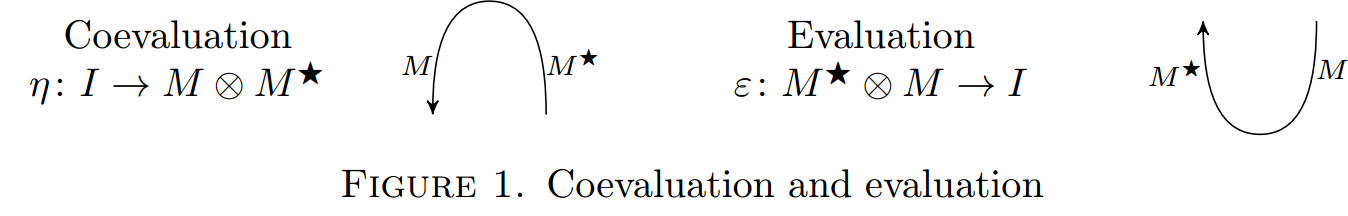
\includegraphics[scale=0.3]{images/ponto-shulman-1}

  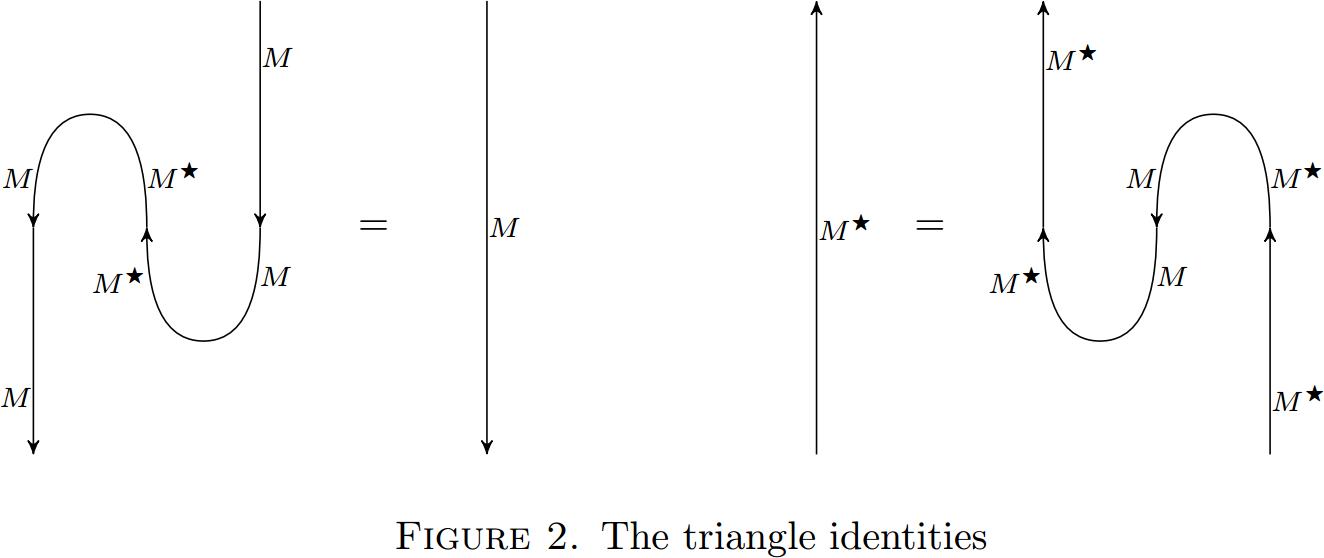
\includegraphics[scale=0.3]{images/ponto-shulman-2}

  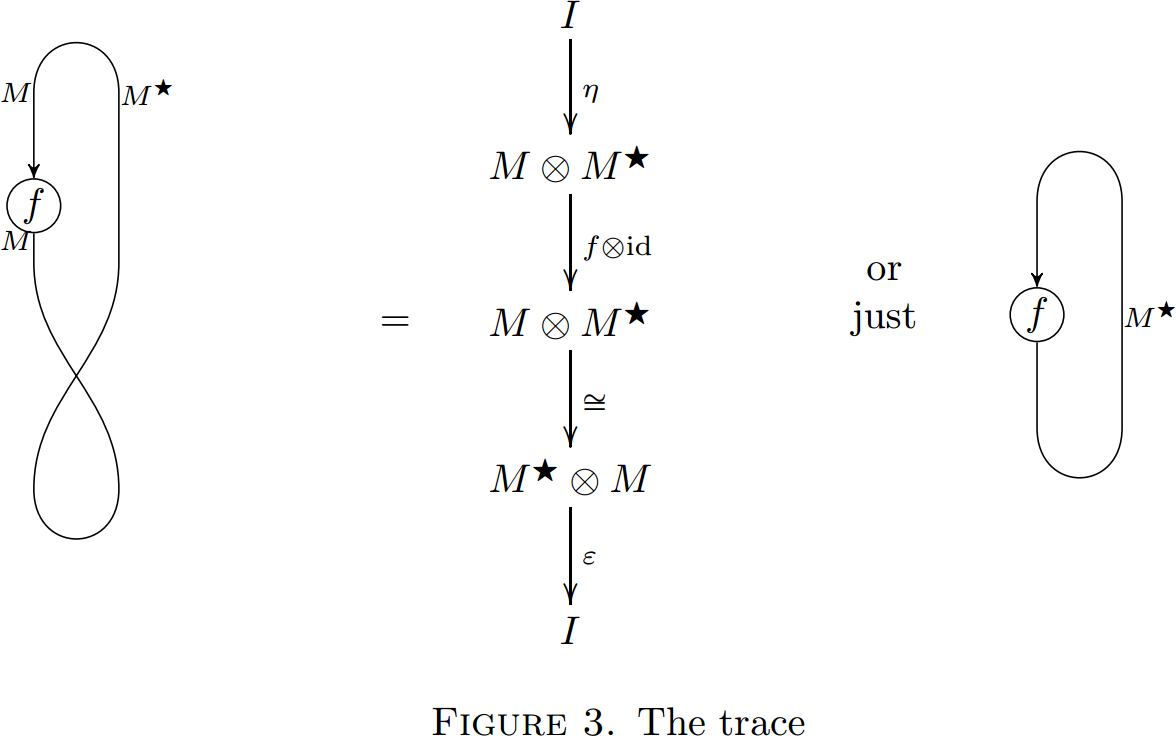
\includegraphics[scale=0.3]{images/ponto-shulman-3}
\end{center}

Um die Begriffe in \textbf{Aufgabe 2c)} zu klären, hilft vielleicht folgende
Skizze (vom Wikipedia-Eintrag zu Kobordismen). Sie illustriert einen Morphismus
von~$S^1$ nach~$S^1 \amalg S^1$.
\begin{center}
  
\includegraphics{images/pair-of-pants}
\end{center}

Hier eine Bemerkung zur Motivation. Das tolle an der Spur-Definition aus der
Aufgabe ist, dass sie in vielen Situationen anwendbar ist und viele Einzelfälle
von Spur-Begriffen vereinigt. Das sind zum einen algebraische Begriffe wie Spur
einer Matrix und Lefschetz-Zahl eines Endomorphismus eines Komplex von
Vektorräumen, zum anderen aber auch Begriffe aus Topologie und
Homotopietheorie. Es gibt einen wunderschönen erklärenden Artikel zum Thema,
den ich euch verlinke, sobald ihr alle das Blatt bearbeitet habt. (In dem
Artikel wird die Aufgabe vollständig gelöst.)

Noch eine Bemerkung für die Gegner von Vektorräumen unter euch: Wer mag, kann
Teilaufgabe~a) auch für Moduln bearbeiten. Allerdings ist nicht jeder Modul
dualisierbar; nur die, die endlich erzeugt und projektiv sind. Das könnte man
auch beweisen. (In diesem Zusammenhang ist interessant, dass ein Modul genau
dann endlich erzeugt und projektiv ist, wenn er \emph{lokal frei} ist;
siehe Marcs Geburtstagsgeschenk auf
\url{https://github.com/iblech/talk-homological-algebra/raw/master/kaplansky-de.pdf}.)

Bei \textbf{Aufgabe 3} soll man sich überlegen, wie die Definitionen
sinnvollerweise auszusehen haben. Welche Isomorphismen sollte man fordern?
Welche Gleichheiten zwischen Morphismen?

\end{document}
